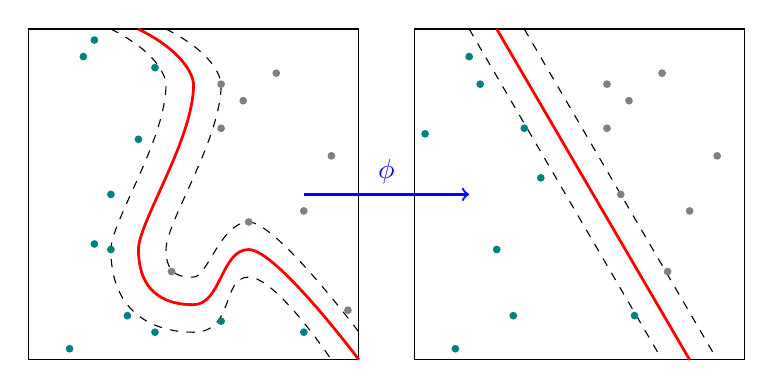
\begin{tikzpicture}[scale=0.7]
  
%draw[color=gray] (0,0) grid (6,6);
\draw (0,0) rectangle (6,6);
% \draw line
\draw[color=red,line width=1pt]
  (2,6) .. controls (3,5.5) and (3,5) .. 
  (3,5) .. controls (3,4) and (2,2.5) .. 
  (2,2) .. controls (2,1) and (2.8,1) .. 
  (3,1) .. controls (3.5,1) and (3.5,2) .. 
  (4,2) .. controls (4.5,2) and (6,0) .. 
  (6,0);
% \draw left dashed line
\draw[dashed] 
  (1.5,6) .. controls (2.5,5.5) and (2.5,5) .. 
  (2.5,5) .. controls (2.5,4) and (1.5,2.5) .. 
  (1.5,2) .. controls (1.5,.5) and (2.8,.5) .. 
  (3,.5) .. controls (3.75,.5) and (3.5,1.5) .. 
  (4,1.5) .. controls (4.5,1.5) and (5.5,0) .. 
  (5.5,0);
% \draw right dashed line
\draw[dashed] 
  (2.5,6) .. controls (3.5,5.5) and (3.5,5) .. 
  (3.5,5) .. controls (3.5,4) and (2.5,2.5) .. 
  (2.5,2) .. controls (2.5,1.5) and (2.8,1.5) .. 
  (3,1.5) .. controls (3.25,1.5) and (3.5,2.5) .. 
  (4,2.5) .. controls (4.5,2.5) and (6,0.5) .. 
  (6,0.5);
%\draw[color=gray] (2,6) -- (3,5) -- (2,2) -- (3,1) -- (4,2) -- (6,0);
%\draw[color=gray] (1.5,6) -- (2.5,5) -- (1.5,2) -- (3,.5)-- (4,1.5)-- (5.5,0);
%\draw[color=gray] (2.5,6) -- (3.5,5) -- (2.5,2) -- (3,1.5)-- (4,2.5)-- (6,0.5);
  
%\draw[color=gray] (7,0) grid (13,6);
\draw (7,0) rectangle (13,6);
% \draw line
\draw[color=red,line width=1pt] (8.5,6) -- (12,0);
% \draw dashed line
\draw[dashed]  (8,6) -- (11.5,0);
\draw[dashed]  (9,6) -- (12.5,0);
  
\draw[thick, ->, blue] (5,3) -- (8,3) node [above,pos=.5] {$\phi$};
  
\def\positive{{%
{2.3,5.3},
{3.5,.7},
{1.5,2},
{1.2,2.1},
{1.8,.8},
{1,5.5},
{1.2,5.8},
{.75,.2},
{2,4},
{5, 0.5},
{1.5,3},
{2.3,.5},
%
{9.3,3.3},
{11,.8},
{8.5,2},
{7.2,4.1},
{8.8,.8},
{8,5.5},
{8.2,5},
{7.75,.2},
{9,4.2},
{12, 0.5},
{8.5,3},
{9.3,.5},
}}
  
% \draw positive dots
\foreach \i in {0,...,20} {
  \pgfmathparse{\positive[\i][0]}\let \x \pgfmathresult;
  \pgfmathparse{\positive[\i][1]}\let \y \pgfmathresult;
  \fill[teal] (\x,\y) circle (2pt);
}
  
\def\negative{{%
{4,2.5},
{3.5,5},
{2.6,1.6},
{4.5,5.2},
{5.5,3.7},
{3.9,4.7},
{5,2.7},
{3.5,4.2},
{5.8,.9},
%
{10.75,3},
{10.5,5},
{11.6,1.6},
{11.5,5.2},
{12.5,3.7},
{10.9,4.7},
{12,2.7},
{10.5,4.2},
{12.8,.9},
}}
  
% \draw negative dots
\foreach \i in {0,...,16} {
  \pgfmathparse{\negative[\i][0]}\let \x \pgfmathresult;
  \pgfmathparse{\negative[\i][1]}\let \y \pgfmathresult;
  \fill[gray] (\x,\y) circle (2pt);
}
  
\end{tikzpicture}
\end{center}